\begin{document}
\title{The $(3,4,\infty)$ family of complex six-spheres\\[.5em]V. Complex fourfolds from the family}
\author{AI-produced mathematical text}
\date{20 November 2026}
\maketitle
\begin{abstract}
We construct compact complex fourfolds diffeomorphic, with their complex
orientation, to $3\mathbb{HP}^2\#(-\mathbb{HP}^2)$.
They form a family of complex three-tori over $\mathbb P^1$ with
monodromy in $GL_6(\mathbb Z)$: two multiple fibres, of multiplicities
five and four, and one Kuhn cusp. Its periods come from the exterior
square of the genus-two pencil $y^2=x^5+\lambda^3x+\lambda^4$.
The family is parametrized exactly
by the half-plane $\operatorname{Im}\xi>c_*$, where
$c_*\approx1.09454$ is minus the minimum of an explicit real-analytic
period function.  We compute the Hodge numbers, the tangent
cohomology (the Kuranishi germ is smooth of dimension one) and the
automorphism group $\mathbb C\times\mathbb Z/2$, and we show that the
family extends analytically across no boundary point of its parameter
domain.  We also construct a compact complex fourfold outside Fujiki's
class $\mathcal C$ as a small crepant resolution of the fibre product of
a complex six-sphere with an elliptic surface; give an effective
classification of the integral monodromy data of this kind that yield
three-connected eight-manifolds, all of which are diffeomorphic to
$3\mathbb{HP}^2\#(-\mathbb{HP}^2)$; and describe shifted fibre products
of complex dimension five.
\end{abstract}
\clearpage
\tableofcontents
\clearpage
\section{Results and their proofs in outline}\label{sec:results}
\subsection{The series and this paper}
This paper is the fifth of a series on the holomorphic families built
from the $(3,4,\infty)$ family of torus-fibred complex structures on
$S^6$ \citep{AC26,E26}.  The table gives the main result of each paper
of the series and the papers it uses.
\begin{center}\small
\begin{tabularx}{\textwidth}{@{}lXl@{}}\toprule
Paper & Main result & Uses\\\midrule
I & Exact periods, moduli, fibre strata and the two ends & ---\\
II & Torus-fibred threefolds with $b_1=b_2=0$: the Campana--Demailly--Peternell argument and the sign theorem for all degenerations & I, IV\\
III & Maps from the six-spheres and the manifolds they give & I, II, IV, V\\
IV & Smooth monodromy in $\Theta_7$ & I, II, III, V\\
V & Complex fourfolds on $3\mathbb{HP}^2\#(-\mathbb{HP}^2)$ and a resolved fibre product & I, III, IV\\
\bottomrule\end{tabularx}\end{center}
\subsection{The main theorems}
\hypertarget{tag-03KQ}{}\label{series:V:main-theorems}

\begin{definition}[The period parameter]
\hypertarget{tag-PV14}{}\label{pub:V:parameter}
\StatementRecord{pub:V:parameter}{proved}{PV14}{}
We use the algebraic splitting $\sigma_b$, invariant vector $e$ and
functional $\alpha$ with the exact normalization of
\cref{def:hb,night:P1.15}. For the rank-three bundle $P$ of
\cref{night:P1.5}, put
\[
 F_\xi=(\sigma_b+\xi\alpha e)(P),\qquad
 c_*=-\min h_b,\qquad
 \mathcal U=\{\xi\in\mathbb C:\operatorname{Im}\xi>c_*\},
\]
where $h_b$ is the real-intersection function of \cref{def:hb}.
We write $M_\xi$ for the compact filling of these periods with the
base and fibre conjugation of \cref{rem:V:conjugation-parameter}.
For the imaginary ray we write $M_c=M_{ic}$, with $c>c_*$.
The positive Kuhn fan is fixed throughout this family.
\end{definition}

\hypertarget{main-V-D}{}
\begin{maintheorem}[The oriented diffeomorphism type]
\hypertarget{tag-03KU}{}\label{series:V:D}
\StatementRecord{series:V:D}{proved}{03KU}{\cref{maps:src:F.3.7}, \cref{maps:src:F.4.1}}
For every $\xi\in\mathcal U$, the genus-two periods of
\cref{series:V:C}, with the integral datum of
\cref{pub:V:rank-six-data}, extend over the finite root charts
and the positive marked Kuhn cusp. They give a compact complex
fourfold $M_\xi$ and an orientation-preserving diffeomorphism
\[
 M_\xi\ \cong\ 3\mathbb{HP}^2\#(-\mathbb{HP}^2).
\]
The fourfolds form a holomorphic family over $\mathcal U$.
Their smooth middle lattice and spin characteristic vector are
isometric to $\bigl(I_{3,1},(1,1,1,1)\bigr)$.
\end{maintheorem}

\textit{Mechanism.} The middle-lattice isometry transports both Euler and Pontryagin clutching data, after which the cited absorption theorem removes the homotopy sphere.
\textit{Relation to literature.} The compact complex realization is new; the smooth classification and absorption results used to identify its underlying manifold are listed in \S\ref{pub:V:known-new}.
\hyperlink{outline-V-D}{Outline of the proof}.

\hypertarget{main-V-E}{}
\begin{maintheorem}[The exact family and its two ends]
\hypertarget{tag-03KV}{}\label{series:V:E}
\StatementRecord{series:V:E}{proved}{03KV}{\cref{night:P1.18}, \cref{night:P1A.1}, \cref{night:P1A.2}, \cref{night:P1A.3}, \cref{night:P1A.4}, \cref{night:P1A.5}, \cref{night:P1.17}, \cref{night:P1A.6}}
Put
\[
 c_*=-h_{b,\min}=\frac{96}{625\pi}\operatorname{Re}(XH_\infty)_{03},
 \qquad \mathcal U=\{\xi\in\C:\Im\xi>c_*\},
\]
where $X$ is the normalized integral intertwiner of
\cref{night:P1.15} and $H_\infty$ is its regular infinity-root
fundamental-solution limit, normalized at $\lambda=1$ as in
\cref{night:P1.18}. Thus
\[c_*\approx1.09454.\]

The marked family is parametrized exactly by $\mathcal U$:
its members are pairwise nonisomorphic, have algebraic dimension one
and automorphism group $\mathbb C\times\mathbb Z/2$, and admit no
antiholomorphic isomorphism for this fan.  The real-intersection
function determines the parameter domain; the invariant line and
one half-period determine the automorphisms, while the reflected cusp map fails to preserve a ray of the chosen fan.
On the effective root curve put
$L=\OO((4/5)[\infty]-(3/4)[0])$. Then
\[
 R^qh_*\OO=\bigwedge^q(\OO\oplus L^{-1}\oplus L^{-2}),
 \qquad K_M=h^*L^{-6}.
\]
With $p$ indexing rows and $q$ indexing columns, the Hodge table is
\[
\begin{array}{c|ccccc}
h^{p,q}&0&1&2&3&4\\\hline
0&1&1&0&0&0\\
1&0&2&1&0&0\\
2&0&1&6&1&0\\
3&0&0&1&2&0\\
4&0&0&0&1&1
\end{array}
\]
The tangent tuple is $h^q(T_M)=(1,1,1,2,0)$ and its Kuranishi germ
is smooth of dimension one. A full parameter disc across the
transversality boundary has the proper-filling obstruction of
\cref{night:P1A.5}. A proper smooth family on a punctured disc
whose fibres belong to $\mathcal U$ has the smooth filling after
the explicit degree-two torsor cover of \cref{night:P1A.6}.


\end{maintheorem}

\textit{Mechanism.} The normalized Frobenius period minimum fixes the exact domain, and the marked period and cap maps determine the family invariants and isomorphisms.
\textit{Relation to literature.} The exact parameter domain and the family invariants are new; the cited direct-image and torus-deformation inputs are listed in \S\ref{pub:V:known-new}.
\hyperlink{outline-V-E}{Outline of the proof}.

\hypertarget{main-V-C}{}
\begin{maintheorem}[The genus-two period construction]
\hypertarget{tag-03KT}{}\label{series:V:C}
\StatementRecord{series:V:C}{proved}{03KT}{\cref{night:P1.4}, \cref{night:P1.5}, \cref{maps:src:F.3.5}, \cref{maps:src:F.3.6}, \cref{night:P1.18}}
The pencil $y^2=x^5+\lambda^3x+\lambda^4$ has one nodal
fibre away from $0,\infty$, at $\lambda_*=-256/3125$.
Its good root charts have orders eight and five, and on that root
curve its Hodge bundle is
\[
 \mathcal H=T^3\oplus T,\qquad
 T=\OO((2/5)[\infty]-(3/8)[0]),\qquad \deg T=1/40.
\]
The meromorphic differential $dx/y$ generates $\ell_0=T^3$.
In the full rank-four de Rham bundle, projection of
$\ell_0\wedge\mathcal H_{\rm dR}$ to
$\bigwedge^2\mathcal H_{\rm dR}/\mathbb C\omega$
is a rank-three bundle $P$.  Its holomorphic lift to the rank-six extension is $(\sigma_b+\xi\alpha e)(P)$, with the
normalization of $e,\alpha,\sigma_b$ in \cref{night:P1.15}.
It is transverse to its conjugate on the completed base exactly
for the parameters $\xi\in\mathcal U$ of Theorem~\ref{series:V:E}.
The exterior-square and lift maps descend the finite root
orders to five and four; the cusp has period
$Z(q)=(\log q/(2\pi i))I_3+C(q)$ with $C$ holomorphic at zero
(\cref{night:P1.4,night:P1.5,maps:src:F.3.5,maps:src:F.3.6,night:P1.18}).

\end{maintheorem}

\textit{Mechanism.} The wedge image of the genus-two Hodge line has rank three, and its split lift becomes transverse after the normalized imaginary shift.
\textit{Relation to literature.} The pencil, its integral exterior-square comparison and its normalized lifted planes are new.
\hyperlink{outline-V-C}{Outline of the proof}.

\hypertarget{main-V-B}{}
\begin{maintheorem}[The integral rank-six construction]
\hypertarget{tag-03KS}{}\label{series:V:B}
\StatementRecord{series:V:B}{proved}{03KS}{\cref{maps:src:F.2.5}, \cref{maps:src:F.2.6}, \cref{night:P1.13}}
The rank-six integral monodromy of \cref{pub:V:rank-six-data}, with free affine fillings of orders five and four and the index-one Kuhn cusp, gives a closed smooth eight-manifold that is three-connected, has free integral homology, and has middle intersection form $3\langle1\rangle\oplus\langle-1\rangle$.

\end{maintheorem}

\textit{Mechanism.} In the integral Leray spectral sequence over $\mathbb P^1$, each order-two suspension class from the order-four filling transgresses to the corresponding nonzero global coinvariant, so the resulting homology is free; Todd integrality and the signature bound then force the middle form.
\textit{Relation to literature.} The integral rank-six datum and its global homology calculation are new; the toroidal filling is the cited construction listed in \S\ref{pub:V:known-new}.
\hyperlink{outline-V-B}{Outline of the proof}.

\hypertarget{main-V-F}{}
\begin{maintheorem}[The integral input classification]
\hypertarget{tag-03KW}{}\label{series:V:F}
\StatementRecord{series:V:F}{proved}{03KW}{\cref{maps:src:F.2.39}, \cref{maps:src:F.3.11}, \cref{maps:src:F.3.4}}
Let $k\in\{2,3\}$ and $\Lambda=\mathbb Z^6$.
Consider ordered integral tuples $(M_1,\ldots,M_k,M_0)$ with each
$M_i$ of finite order and having a nonzero fixed vector, with
$M_0=(M_1\cdots M_k)^{-1}$, and with
$N=M_0-I$ satisfying $N^2=0$, rank three, and
$\operatorname{im}N=\ker N$ as integral sublattices of $\Lambda$.
Every such tuple has a computable canonical representative and an
explicit simultaneous unimodular conjugator; equality of the
representatives is equivalent to simultaneous integral conjugacy.
For input entry height $H$, the finite stopping bound is
$(2H+1)^{36(k+1)}$ candidates before the proved rejection filters.
The ordered sector with both finite linear orders two has exactly
56 classes.  Each has free affine lifts of affine order four,
and every free affine filling of this sector has nontrivial
fundamental group.

Specify the free affine actions
$\tau_i(x)=M_ix+v_i/m_i$, with $v_i\in\Lambda$ and affine order $m_i$, an integral translation clutch $\kappa\in\Lambda$,
and a primitive Kuhn cusp marking.  The algorithms compute the
full fundamental group and every integral homology group of the
resulting marked gluing for every such input.  Their constructive
parametrization and finite tests identify exactly the inputs with
$\pi_1=1$ and $H_2=H_3=0$; there is no fixed bound on the
orders, twists or lattice indices (\cref{maps:src:F.2.39}).
Every resulting three-connected manifold is orientation-preservingly
diffeomorphic to $3\mathbb{HP}^2\#(-\mathbb{HP}^2)$, by
\cref{maps:src:F.2.30}.

On $B^*=\mathbb P^1\setminus\{p_0,\ldots,p_k\}$ with $k\ge1$,
every representation $\rho:\pi_1(B^*)\to GL^+(6,\mathbb R)$
whose $p_0$ monodromy satisfies $(M_0-I)^2=0$ and
$\operatorname{rank}(M_0-I)=3$ has a holomorphic period family
transverse to its conjugate everywhere on $B^*$. In the marking
$M_0=\left(\begin{smallmatrix}I&I\\0&I\end{smallmatrix}\right)$,
its cusp period is
\[
 Z(t)=\frac{\log t}{2\pi i}I_3+C(t),\qquad C\text{ holomorphic at }0,
\]
with any prescribed finite jet of $C$ at zero. An integral primitive
cusp admits an integral marking. The other $p_i$ remain punctures
in this assertion (\cref{maps:src:F.3.11}).

For a polarized algebraic abelian-surface family with toric-rank-two
cusp, the construction that takes a fibrewise degree-zero line bundle
and quotients its punctured bundle by a lifted translation cannot
have $b_1=b_2=0$ with the stipulated rank-three square-zero Kuhn
cusp; this holds for both proportional and nonproportional source
sections. The filtration and Euler-parity proof is
\cref{maps:src:F.3.4}.

\end{maintheorem}

\textit{Mechanism.} Exact intertwiner lattices decide simultaneous conjugacy, finite integral complexes compute each marked gluing, and the cusp-period construction realizes the punctured analytic data.
\textit{Relation to literature.} The classification and bounded-cusp period theorem are new; their cited lattice-isomorphism and Oka inputs are listed in \S\ref{pub:V:known-new}.
\hyperlink{outline-V-F}{Outline of the proof}.


\hypertarget{main-V-A}{}
\begin{maintheorem}[The resolved transverse elliptic fibre product]
\hypertarget{tag-03KR}{}\label{series:V:A}
\StatementRecord{series:V:A}{proved}{03KR}{\cref{maps:src:E.1.2}, \cref{maps:src:E.2.1}}
Let $X$ be a canonical marked member of the $(3,4,\infty)$
family, with reduced multiple fibres $S_1,S_2$ of multiplicities
three and four, and put $L=\mathcal O_X(S_1-S_2)$.
Let $S\to\mathbb P^1$ be the elliptic surface in
\cref{maps:src:E.1.2}, with its cusp over the cusp of $X$.
The fibre product $X\times_{\mathbb P^1}S$ has the small
crepant resolution $\Pi:Z\to X$ of that theorem.
It is a compact complex fourfold with
$K_Z=\Pi^*L^{-5}$, algebraic dimension two,
$b_1(Z)=0$, and $h^{0,1}(Z)=1$.
Its signature is two and its middle intersection form is
$\langle1\rangle\oplus\langle1\rangle$.
It lies outside Fujiki's class $\mathcal C$.
\end{maintheorem}

\textit{Mechanism.} The explicit period comparison and a small crepant Kuhn resolution preserve the root canonical calculation and the integral characteristic pairings.
\textit{Relation to literature.} The global small crepant resolution and its computed invariants are new; the cited six-sphere, elliptic and toroidal constructions are the inputs listed in \S\ref{pub:V:known-new}.
\hyperlink{outline-V-A}{Outline of the proof}.

\subsection{The proofs in outline}
\hypertarget{outline-V-D}{}
\subsubsection*{Theorem~\ref{series:V:D}: The oriented diffeomorphism type}
\begin{enumerate}[label=\arabic*.,leftmargin=*]
\item\hypertarget{step-V-D-1}{} The lifted periods commute with the finite root actions and
  have the prescribed bounded cusp correction, so the same quotient
  and toroidal charts are holomorphic and proper.  Their collar
  identifications are the marked maps used in the smooth construction
  (\cref{maps:src:F.3.7}, \cref{night:P1.9}).

\item\hypertarget{step-V-D-2}{} The preceding integral calculation gives the intersection
  lattice $I_{3,1}$.  The spin characteristic vector $p_1/2$ has
  square two, by the Chern-number calculation
  (\cref{night:P1.13}).

\item\hypertarget{step-V-D-3}{} The characteristic vector has odd coordinates and norm two in $I_{3,1}$. The integral reflection in $(1,1,1,1)$ strictly decreases the absolute negative coordinate until all four coordinates have absolute value one. The resulting explicit isometry is proved in \cref{night:P1.13}.

\item\hypertarget{step-V-D-4}{} In the quaternionic clutching coordinates, the map is
  $(a,b)\mapsto(e,p_1/2)=(a-b,a+b)$, with inverse
  $((e+p_1/2)/2,(p_1/2-e)/2)$.  Thus the pairing and characteristic
  vector determine the normal datum; the Poincar\'e-duality map
  transports it with the middle lattice isometry
  (\cref{maps:src:F.4.1}).

\item\hypertarget{step-V-D-5}{} Each quaternionic projective-plane summand has $p_1=2u$.
  The oriented connected-sum pairing and characteristic vector are
  therefore the same pair $\bigl(I_{3,1},(1,1,1,1)\bigr)$.
  Wall's stated extended-form classification gives the oriented
  diffeomorphism up to a homotopy eight-sphere
  (\cref{maps:src:F.4.1}).

\item\hypertarget{step-V-D-6}{} Kramer--Stolz's Theorem~A absorbs that sphere in one positive
  $\mathbb{HP}^2$ summand.  Its diffeomorphism has degree $+1$ because
  the square of a middle generator evaluates to $1$ on both sides.
  Oriented connected-sum maps therefore give the required oriented
  diffeomorphism of the full fourfold
  (\cref{maps:src:F.4.1}).

\end{enumerate}

\hypertarget{outline-V-E}{}
\subsubsection*{Theorem~\ref{series:V:E}: The exact family and its two ends}
\begin{enumerate}[label=\arabic*.,leftmargin=*]
\item\hypertarget{step-V-E-1}{} The infinity-root symmetry makes the differential of the normalized height vanish at zero. Its positive Hessian proves a strict local minimum. Convergent root and cusp expansions, with interval continuation over finite closed covers, prove the height is strictly larger on their complements; the positive cusp graph treats the remaining inner disc. This proves the unique global minimum and the exact domain in \cref{night:P1.18}.

\item\hypertarget{step-V-E-2}{} On the effective root curve of orders five and four put
  $L=\mathcal O((4/5)[\infty]-(3/4)[0])$.  The direct images are
  $R^qh_*\mathcal O=\bigwedge^q
  (\mathcal O\oplus L^{-1}\oplus L^{-2})$, and
  $K_M=h^*L^{-6}$.  The toric normalization complex proves the
  exterior-algebra assertion at the cusp, and the root-chart
  invariant cohomology proves it at the finite fibres
  (\cref{night:P1A.1}).

\item\hypertarget{step-V-E-3}{} The logarithmic cotangent sequence and its explicit residue
  matrices give the Hodge table below.  Serre duality applied to
  the twisted logarithmic and residue sequences gives
  $h^q(T_M)=(1,1,1,2,0)$.  The normal tangent map and the period lift give a nonzero Kodaira--Spencer class; the local
  analytic-ring comparison makes the Kuranishi germ smooth of
  dimension one (\cref{night:P1A.2}, \cref{night:P1A.3}).

\item\hypertarget{step-V-E-4}{} Restriction of a horizontal divisor to a regular torus fibre
  gives an invariant alternating class.  The computed invariant
  space is zero, while positive pairing with a torus Kähler form
  rules out a nonzero effective divisor of zero class.  Thus the
  meromorphic field is the base field $\mathbb C(\lambda)$.
  Every isomorphism therefore preserves the base and its three
  distinguished values.  The simultaneous linear centralizer is
  $\mathbb Q I$; the order-five affine norm excludes its negative
  integral unit.  The translation sheaf has identity component
  $\mathbb C$ and an integral parabolic quotient $\mathbb Z/2$,
  represented by the displayed half-period, proving the
  automorphism group and equality of parameters for isomorphic
  members (\cref{night:P1A.4}).

\item\hypertarget{step-V-E-5}{} The two integral anti-intertwiners are $\pm R$.  One is excluded
  by the finite cap norm.  For the other, the based cusp
  correction acts on rays by $-P$, and takes $e_2$ to $(0,-1,1)$,
  outside the component's rays $\pm(\{0,1\}^3\setminus\{0\})$.
  The corresponding monomial map contracts a divisor, contradicting
  a biholomorphism (\cref{night:P1.17}).

\item\hypertarget{step-V-E-6}{} A proposed proper Hausdorff filling across a boundary point of
  a full parameter disc recovers the marked base from the moving
  pencil of $K_M^{-4}$, whose two sections have ratio $\lambda$.
  Closed relative forms give torus fibres outside a proper
  analytic subset.  Their marked periods continue as $F_\xi$,
  while the real hypersurface $h_b+\operatorname{Im}\xi=0$
  cannot be contained in that analytic subset.  A torus fibre
  there violates real transversality (\cref{night:P1A.5}).  For a family on a punctured disc whose
  fibres belong to $\mathcal U$, the unique classifying map is
  holomorphic; its Cayley transform extends and the maximum principle
  keeps its limit inside $\mathcal U$.  After the explicit degree-two
  removal of the finite torsor, that family has a smooth filling
  (\cref{night:P1A.6}).

\end{enumerate}

\hypertarget{outline-V-C}{}
\subsubsection*{Theorem~\ref{series:V:C}: The genus-two period construction}
\begin{enumerate}[label=\arabic*.,leftmargin=*]
\item\hypertarget{step-V-C-1}{} The pencil has one node at $\lambda_*=-256/3125$ and good
  reductions after root orders eight and five.  Its Hodge bundle on
  that root curve is $T^3\oplus T$, with
  $T=\mathcal O((2/5)[\infty]-(3/8)[0])$ and
  $\deg T=1/40$ (\cref{night:P1.4}).

\item\hypertarget{step-V-C-2}{} In the exterior-square lattice, projection induces
  $j:\omega^\perp\to(\bigwedge^2\mathbb Z^4)/\mathbb Z\omega$
  with Smith factors $(1,1,1,1,2)$.  This exact index-two map identifies
  the rational systems, and the quotient is the dual of the primitive
  integral lattice.  The lower five-dimensional blocks of the given
  rank-six tuple are the quotient blocks under this map
  (\cref{night:P1.2}).

\item\hypertarget{step-V-C-3}{} Put $P=p(\ell_0\wedge\mathcal H_{\mathrm{dR}})$, where
  $\ell_0=\langle dx/y\rangle$ and $p$ is projection modulo $\omega$.
  The wedge map has rank three and its image meets $\mathbb C\omega$
  trivially: a decomposable two-vector has square zero, whereas
  $\omega^2\ne0$.  This proves the required rank before a lift is
  chosen (\cref{night:P1.5}, \cref{maps:src:F.3.5}).

\item\hypertarget{step-V-C-4}{} The root-line decomposition of $P$ has $H^1(P^*)=0$ and a one-dimensional space of functionals by \cref{night:P1.5}. Its extension therefore splits holomorphically. The exact contraction and period comparison in \cref{def:hb} identify the normalization of $\alpha$ and $\sigma_b$.

\item\hypertarget{step-V-C-5}{} For the real-intersection line, the normalized lift has transversality exactly when $h_b+\operatorname{Im}\xi\ne0$. The cusp has $Z=(\log q)/(2\pi i)I_3+C(q)$ and $h_b\to+\infty$. Thus the complete parameter domain is the half-plane above $-\min h_b$, by \cref{night:P1.8,night:P1.18}.

\end{enumerate}

\hypertarget{outline-V-B}{}
\subsubsection*{Theorem~\ref{series:V:B}: The integral rank-six construction}
\begin{enumerate}[label=\arabic*.,leftmargin=*]
\item\hypertarget{step-V-B-1}{} The matrices of \cref{pub:V:rank-six-data} have orders five and four. The square-zero cusp has primitive rank-three image, and its explicit unimodular marking is proved in \cref{night:P1.1}. The invariant covector $x\mapsto x_0$ detects every nonidentity affine power, proving the freeness used in \cref{pub:V:smooth-gluing}.

\item\hypertarget{step-V-B-2}{} The cusp and finite quotient charts give the marked smooth gluing. Its van Kampen relations reduce to $5a=h$, $4b=-h$ and $a+b=0$; their integral relation matrix is unimodular. Hence the manifold is simply connected, by \cref{pub:V:smooth-gluing}.

\item\hypertarget{step-V-B-3}{} The signed-orbit bases at the finite cores, their norm maps, and the primitive cusp collapse give the integral restriction sheaves and their point kernels. Determinant minors compute their cohomology in \cref{pub:V:integral-restrictions}, using the collapse of \cref{night:P1.11}.

\item\hypertarget{step-V-B-4}{} For the order-four core, the loops $v=g^4h^{-1}$ and $t=g$ form an integral basis. A torsion representative pulls back to $(0,w)$, so its transgression is $\pm[w]$ by \cref{mapsaudit:order-four-torsion-transgression}. The three nonzero global images are proved in \cref{pub:V:integral-restrictions}.

\item\hypertarget{step-V-B-5}{} The three torsion differentials are isomorphisms onto $\mathbb Z/2$. The remaining cusp kernel is free of rank one. The Leray filtration, universal coefficients, duality and Hurewicz then give free integral homology and three-connectivity in \cref{maps:src:F.2.6}.

\item\hypertarget{step-V-B-6}{} The almost complex structure has $c_1=c_3=0$. The index and signature identities of \cref{sec:V-known-inputs} force $c_2^2=2$, $\sigma=2$ and the middle form $I_{3,1}$. The Pontryagin identities and characteristic vector are computed in \cref{night:P1.13}.

\end{enumerate}

\hypertarget{outline-V-F}{}
\subsubsection*{Theorem~\ref{series:V:F}: The integral input classification}
\begin{enumerate}[label=\arabic*.,leftmargin=*]
\item\hypertarget{step-V-F-1}{} Primitive square-zero cusp matrices have the explicit integral
  normal form and centralizer
  $\left(\begin{smallmatrix}P&Q\\0&P\end{smallmatrix}\right)$.
  Eigenvalue one is necessary for a free affine lift, leaving the
  finite cyclotomic list and its complex-compatibility filter
  (\cref{maps:src:F.2.1}, \cref{maps:src:F.2.2}).

\item\hypertarget{step-V-F-2}{} The rational intertwiner algebra, its radical and its
  semisimple quotient reduce the simultaneous integral-conjugacy
  problem to the cited lattice-isomorphism algorithm in its verified
  hypothesis.  Searching by height and lexicographic order terminates
  by the input height, yielding a canonical representative and an
  explicit unimodular conjugator (\cref{maps:src:F.2.36}, \cref{maps:src:F.2.37}).

\item\hypertarget{step-V-F-3}{} For that conjugator $R$, the coordinate map $x\mapsto Rx$
  transports $(M_i,v_i,\kappa,P)$ to
  $(RM_iR^{-1},Rv_i,R\kappa,RP)$.  Since
  $(RP)^{-1}(Rx)=P^{-1}x$, it intertwines the cusp charts
  as well as the affine caps and clutch.  The resulting finite
  cellular cone and group presentation compute all integral homology
  and the full fundamental group (\cref{maps:src:F.2.31}, \cref{maps:src:F.2.35}, \cref{maps:src:F.2.39}).

\item\hypertarget{step-V-F-4}{} The exact two-point tests and the three-point
  orbifold quotient give the complete constructive parametrization;
  the separate involution branch has 56 classes.  The displayed
  unbounded trace family shows why the terminating bound depends on
  the input (\cref{maps:src:F.2.30}, \cref{maps:src:F.2.38}, \cref{maps:src:F.2.39}).

\item\hypertarget{step-V-F-5}{} Nine explicitly given complex-line directions and a uniform
  singular-value bound put a spanning tube in the unpolarized period
  domain.  The local-spray approximation theorem, with the
  relative extension-point argument proved here, produces a
  holomorphic transverse period section and retains any prescribed
  bounded cusp jet (\cref{maps:src:F.3.8}, \cref{maps:src:F.3.10}, \cref{maps:src:F.3.11}).

\item\hypertarget{step-V-F-6}{} For a polarized abelian-surface source, semisimplicity and the
  maximal square-zero cusp force the middle rank-four system to have
  no invariant or coinvariant vectors.  The filtration
  $0\subset\mathbb Q\subset E\subset T$, with middle quotient that
  system and top quotient $\mathbb Q$, then forces both relevant
  invariant ranks to be one; the integral Euler-parity relation
  excludes $b_1=b_2=0$ (\cref{maps:src:F.3.4}).

\end{enumerate}

\hypertarget{outline-V-A}{}
\subsubsection*{Theorem~\ref{series:V:A}: The resolved transverse elliptic fibre product}
\begin{enumerate}[label=\arabic*.,leftmargin=*]
\item\hypertarget{step-V-A-1}{} Pull back the Weierstrass family to the root curve of the
threefold fibration.  The integral matrices $A,B$ give the period comparison $AZ_3B^{-1}=\operatorname{diag}(Z_2,s+c_E)$.
See \cref{maps:src:E.1.2}.
\item\hypertarget{step-V-A-2}{} The unimodular Kuhn fan resolves the local fibre product
without adding rays.  Its period action is proper and its marked
section extends face by face.  The resolution is therefore small
and crepant.
See \cref{maps:src:E.1.2}.
\item\hypertarget{step-V-A-3}{} The canonical formula on the root curve gives
$K=\Pi^*L^{-5}$.  The split relative elliptic complex and Leray
give $(h^{0,q})=(1,1,0,0,0)$; the explicit meromorphic product
comparison gives algebraic dimension two.
See \cref{maps:src:E.2.1}.
\item\hypertarget{step-V-A-4}{} A K\"ahler modification in class $\mathcal C$ preserves
$b_1$ and $h^{0,1}$.  Here $b_1=0$ and $h^{0,1}=1$, contradicting
the K\"ahler equality $b_1=2h^{0,1}$.  This proves the stated
exclusion through these invariants.
See \cref{maps:src:E.2.1}.
\item\hypertarget{step-V-A-5}{} The universal Todd and Pontryagin formulas give
$c_2^2=2$, $c_4=6$ and signature two.  The middle lattice is
positive definite unimodular of rank two, hence has the displayed
form.  
See \cref{maps:src:E.2.1}.
\end{enumerate}

\subsection{Known and new}\label{pub:V:known-new}
\begin{center}\small
\begin{tabularx}{\textwidth}{@{}lX@{}}\toprule
Theorem & Status and principal cited inputs\\\midrule
\ref{series:V:D} & New compact complex realization. Smooth classification: \cite[Definition~3.6 and Theorem~3.7(1), arXiv v3, pp.~12--14]{IVVWallForm}; sphere absorption: \cite[Theorem~A, p.~178]{IVVKramerStolz}; connected-sum criterion and tangent classes: \cite[Corollary~1.4, p.~4, Lemma~2.1, p.~5, and Theorem~2.4, p.~7]{ffMandal}.\\
\ref{series:V:E} & New parameter domain and invariants. Weighted-base and direct-image method: \cite[Lemmas~6.1--6.2, pp.~74--75, Proposition~6.10, pp.~79--80]{DGKX2026v1}; torus deformations: \cite[Theorem~2.1, p.~264]{Catanese2004}.\\
\ref{series:V:C} & New genus-two pencil and integral lifted-period construction. The cusp model is \cite[Theorem~8.7, arXiv v1, pp.~57--59]{Yang2026}.\\
\ref{series:V:B} & New integral rank-six gluing and homology. Toroidal filling and Euler number: \cite[Theorem~8.7 and Corollary~8.8, arXiv v1, pp.~57--59]{Yang2026}; integral specialization: \cite[\S7.7, pp.~60--63]{AC26}.\\
\ref{series:V:F} & New integral classification and period theorem. Lattice isomorphism: \cite[Theorem~3.4, p.~6, Algorithm~8.3, p.~21]{rootBHJ22}; local-spray approximation: \cite[Proposition~7.13 and preceding paragraph, arXiv v5, pp.~23--24]{IVVOkaOneV5}.\\
\ref{series:V:A} & New small crepant resolution and its invariants. Six-sphere: \cite[Theorems~7.17 and~7.22, pp.~57 and~60]{AC26}; elliptic surface: \cite[\S2, arXiv v1, p.~3]{E26}; characteristic identities: \cite[(1.2)--(1.4), pp.~3--4]{ffEsoleKang}; class-$\mathcal C$ criterion: \cite[Theorem~1.1, Remark~1.2, p.~2]{ffJiaMeng}.\\
\bottomrule\end{tabularx}\end{center}
\subsection{Methodology}
This text is AI-produced; no part of it was written by a human.
GPT-5.6 Sol (OpenAI), in Codex at reasoning effort ultra, wrote the
working edition on 24 August--9 September 2026. GPT-6 Astra (OpenAI),
in ChatGPT Pro mode, carried out the research of 12--16 November,
the independent re-derivation of 16--18 November, and the writing of
16--20 November 2026. The publication revision and further checks of
this paper were undertaken by GPT-6 Astra on 20 November 2026.
The reasoning-effort setting of this publication session was inherited;
the interface exposed no separate numerical setting.

Claude Fable 5.2 (Anthropic), at effort high and at effort max, and
Claude Opus 5.5 (Anthropic), at effort max, undertook readings, intakes,
checks and recomputations on 12--20 November 2026. Their objections
and calculations were compared with the statements, proofs and cited
sources, and the resulting corrections were incorporated into the text.
The records specify the passages and calculations examined by each model.

For the statements printed in this paper, the record contains
334 examinations of proof steps, 45 independent re-derivations, and
161 computations or formal certificates. It contains another eight
proof examinations and three re-derivations associated specifically
with steps of the introductory outlines. Each total sums recorded
links from a check to a statement, so one calculation applied to several
statements can contribute several links. Each outcome states the part
examined. The 252 readings associated with the current statements are
recorded separately. Numerical interval enclosures are accompanied by
an independently implemented numerical comparison and exact checks of
the finite covering and sign inequalities. Their respective scopes are
given in the records. No human has checked the mathematics.

The historical sources, programs and check records are available in the
\href{https://github.com/KokunoYumeto/s6-complex-structure-workbench/tree/\SsixRepositoryCommit/pro_returns/S6_SERIES_GRIND_checkpoint_10_20261120T0211Z/}{project repository}.
The additional records and programs of this publication revision
accompany its source distribution.
The text and accompanying work are dedicated to the public domain under
\href{https://creativecommons.org/publicdomain/zero/1.0/}{CC0 1.0 Universal}.

\subsection{How the paper is organized}
Part~\ref{pub:V:part-rank-six} constructs the marked rank-six family.
The local monodromy and cusp in \S\ref{pub:V:sec-local} precede the
period planes in \S\ref{pub:V:sec-periods}, the integral homology in
\S\ref{pub:V:sec-integral}, and the oriented smooth classification
in \S\ref{pub:V:sec-diffeomorphism}. Sections
\ref{pub:V:sec-parameter}--\ref{pub:V:sec-boundary} determine its
parameter domain, invariants and boundary.
Part~\ref{pub:V:part-classification} classifies the integral data and
constructs punctured-base periods. Part~\ref{pub:V:part-resolved}
gives the resolved elliptic fibre product. Part~\ref{pub:V:part-shifted}
uses the sphere fibrations to construct shifted fivefolds and determines
their integral homotopy and smooth topology.

\begin{figure}[htbp]\centering
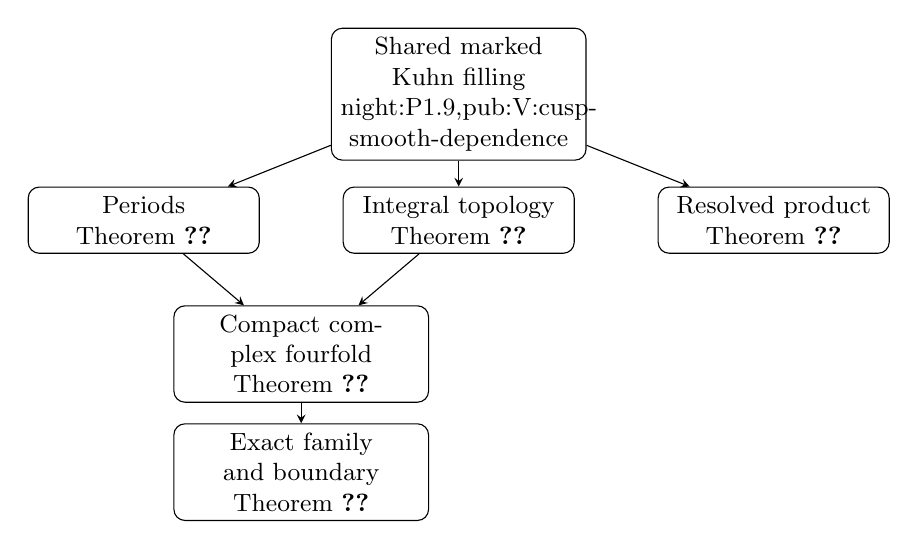
\begin{tikzpicture}[>=stealth,every node/.style={font=\small,align=center}]
\node[draw,rounded corners,text width=3cm] (local) at (0,0) {Shared marked Kuhn filling\\\cref{night:P1.9,pub:V:cusp-smooth-dependence}};
\node[draw,rounded corners,text width=2.7cm] (period) at (-4,-1.6) {Periods\\Theorem~\ref{series:V:C}};
\node[draw,rounded corners,text width=2.7cm] (topology) at (0,-1.6) {Integral topology\\Theorem~\ref{series:V:B}};
\node[draw,rounded corners,text width=2.7cm] (resolved) at (4,-1.6) {Resolved product\\Theorem~\ref{series:V:A}};
\node[draw,rounded corners,text width=3cm] (compact) at (-2,-3.3) {Compact complex fourfold\\Theorem~\ref{series:V:D}};
\node[draw,rounded corners,text width=3cm] (family) at (-2,-4.8) {Exact family and boundary\\Theorem~\ref{series:V:E}};
\draw[->] (local)--(period);\draw[->] (local)--(topology);\draw[->] (local)--(resolved);
\draw[->] (period)--(compact);\draw[->] (topology)--(compact);\draw[->] (compact)--(family);
\end{tikzpicture}
\caption{The shared marked cusp and the main construction. The general classification of Theorem~\ref{series:V:F} is developed separately in Part~\ref{pub:V:part-classification}.}
\end{figure}

\subsubsection*{Further results}
\begin{itemize}[leftmargin=*]
\item \Cref{maps:src:E.2.3,maps:src:E.2.6}: the shifted fivefold has a torus-knot peripheral presentation and explicitly computed integral homology.
\item \Cref{maps:src:E.2.7,maps:src:E.2.9}: all transverse shifts have one oriented smooth type and are framed null-bordant over their fundamental group.
\item \Cref{maps:src:E.2.11,maps:src:E.2.17}: the cusp and peripheral maps determine the full second-homotopy module and its coinvariants.
\item \Cref{maps:src:E.2.13,maps:src:E.2.14}: a circle fibration has an infinite-order return map given by the separating torus twist.
\item \Cref{maps:src:E.2.19,maps:src:E.2.21}: the relative cusp model gives an explicit smooth framed-handle presentation.
\end{itemize}

\clearpage
